\documentclass[a4paper]{article}

\usepackage[english]{babel}
\usepackage[utf8]{inputenc}
\usepackage{amsmath}
\usepackage{graphicx}
\usepackage{hyperref}
\hypersetup{
    colorlinks=true,
    citecolor=blue,
    linkcolor=blue,
    urlcolor=blue
}

\usepackage{biblatex}
\addbibresource{references.bib}

\title{Disease Diagnosis with AI}

\author{Rishit Dagli \\ 
        10 Grade, Thakur International School \\
        \href{mailto:rishit.dagli@gmail.com}{rishit.dagli@gmail.com} }
\date{}

\begin{document}

\maketitle

\section{The problem statement}

In this project I majorly aim to show how we can use Machine Learning to diagnose diseases at an early stage. The problem which I am focusing on is high deaths globally due to diseases like COVID, Tuberculosis or Pneumonia. There have been over 843 K deaths due to COVID (From Google News), deaths due to Pneumonia \& Tuberculosis are very high too. This may be possible with some sensor data which could monitor a persons' vitals or from some test. However, in this project I particularly demonstrate using Machine Learning on chest X-Rays to predict if a person may have COVID using Computer Vision techniques made easy with \href{https://cloud.google.com/automl}{Google Cloud Auto ML}.

\subsection{Early diagnosis}

\qquad A major reason behind being unable to treat diseases like pneumonia, cancer or other such acute diseases is due to them being diagnosed at a very later stage. Major aims under this domain would be to diagnose diseases at a very early stage before it's progression to $3^{rd}$ or $4^{th}$ stage from tests or reports. Early diagnosis of diseases can work as key to success in recovery. As an example, just pneumonia accounts for 1.4 million deaths in children worldwide each year. A lot of these deaths could well be prevented with premature diagnosis. 

\subsection{Easier diagnosis}

\qquad Disease Diagnosis with AI also makes it very easy to receive diagnosis by just uploading for example image of an eye to diagnose eye disease, a CT scan, an X-Ray, chest X-Rays in this case or some other reports in a mobile or web-app to very easily diagnose diseases. It also allows to get faster diagnosis. People can at their homes or local healthcare center itself perform diagnosis for diseases. Since, this would make it very easy to diagnose diseases it would considerably reduce the death rate due to these diseases.

\subsection{Accurate diagnosis}

\qquad In most cases AI algorithms could make better predictions than experts in the field too. However, at this stage I have not tested the model made by me with experts in the field as of now. But in a lot of cases AI could outperform the experts as it could find some spuriously correlated features in the images. While trying to increase the accuracy of the model I also make sure to reduce the False Positives from the model as they could particularly be harmful for the disease diagnosis scenario. With the help of expert medical practitioner I can adapt it to different medical situations.

\qquad So, I feel that if such a system is implemented it would be very beneficial for a lot of people. My own grandmother suffers from an acute disease which has now reached the stage where it cannot be treated. The cause behind this is that it was diagnosed late. seeing this myself I got the inspiration to build an easy diagnosis system which could help in such cases. This is why I chose to work on this problem.

\section{How AI helps to solve this}

\qquad The data I use as mentioned earlier is of chest X-Rays of COVID and normal patients. I try to then find some features from these images using Machine Learning. I pass in this data to \href{https://cloud.google.com/vision/automl/docs}{Google Cloud Auto ML Vision} which then helps me by training an ML algorithm on this. It also helps me to easily deploy my model to a web service which can be used by doctors for easy diagnosis or can also be used by people. I feel this would specially help in this pandemic times when particularly in India there are not enough doctors to even diagnose diseases specially in the COVID times.

\qquad Since most people posses smartphones I have also made an Android application with Auto ML model trained for the edge. I use the `.tflite` model file generated by Auto ML and use this to make the deployment on an Android app. To make the application creation part easier I also use the Android Studio Machine Learning Model Binding Plugin with Android 11 and beta release of Android Studio 4.1. This allows me to use the `tflite` model with just a few lines of code in my Android application. This would considerably make consuming the model by the users very easy, since they could just download an app and do so. To make the process of capturing and working with the X-Ray images easier I use `CameraX` to do so. I have also included the source code for the Android application in the repository made by me for this submission.

\qquad As of now I have not made a production ready Android application and just a proof of concept to demonstrate that edge deployments for this use-case could be made. With support from Google Code To Learn I plan to mainly include the ideas of Federated Learning in the application considering that this is a sensitive application and the features to identify a disease may change. So, there would be a requirement of retraining the model on edge without affecting the privacy of the users.

\qquad Google Cloud Auto ML also allows me to very easily deploy model to the web, this web application could be given to the doctors from where they could make diagnosis and also enter new users data which could help update the model constantly improving the performance of it. As highlighted earlier in this document making updates to the model and improving it in a sensitive use-case like this would be very important.

\subsection{The process used}

\qquad I use a very simple process to build the AI algorithm. I first explore a small set of my data to understand the data. To make sure that there are distinctive features in this small subset of the data, I make use of Keras (tf.keras) to implement a couple of convolutional layers which help me understand the global level features in the images. Being successful in finding some distinctive features in the images.

\qquad I then use this subset of randomly selected images with Auto ML to present a proof that such a method would work as shown in the accompanying video submission. Having validated this, I use the complete set of images with Auto ML Vision to create an AI algorithm that could work in predicting new images if they are normal patients or COVID patients.

\section{The data used}

\qquad I use open-sourced Chest X-Rays images for COVID-19. The image data is collected from public sources only. As for the data I have referenced the paper - COVID-19 image data collection (Joseph Paul Cohen et al.) \cite{cohen2020covid19}. The images and data have been released publicly released at \cite{cohen2020covid} -  \href{https://github.com/ieee8023/covid-chestxray-dataset}{github.com/ieee8023/covid-chestxray-dataset}. The author has scraped the data from multiple websites majorly from - 
\begin{itemize}
    \item \href{https://radiopaedia.org/}{radiopaedia.org}
    \item \href{https://www.sirm.org/category/senza-categoria/covid-19/}{sirm.org}
    \item \href{https://www.eurorad.org/}{eurorad.org}
    \item \href{https://coronacases.org/}{coronacases.org}
\end{itemize}

\qquad I have also used some pretty basic transformations on the image to better run the algorithms. I use $382$ labelled images in all. These are then split into $3$ sets - Train, validation and test sets according to $8:1:1$ ratio. So, I use -
\begin{itemize}
    \item $306$ images for training
    \item $38$ images for validation
    \item $38$ images for test
\end{itemize}

\section{Materials}

\qquad The codes, submission video and the Android application for this project are available at: \cite{CodeToLearnGH} \href{https://github.com/Rishit-dagli/Code-to-Learn-2020}{github.com/Rishit-dagli/Code-to-Learn-2020}

\section{Model Metrics}

The Fig. \ref{fig:1} shows the trained model metrics, with Auto ML I receive a good precision and recall of $97.37$ \%

%\begin{figure}[ht]
%  \centering
%  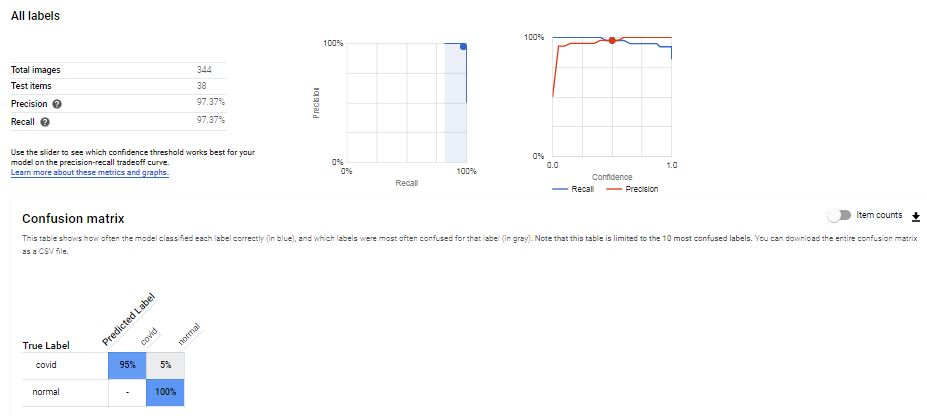
\includegraphics[width=\linewidth]{metrics.JPG}
  %\captionsetup{justification=raggedright}
%  \caption{Model Metrics}
%  \label{fig:1}
%\end{figure}

\section{Future additions}

\qquad In this project I have worked only on the ML part, but a real-life solution needs to be made in collaboration with medical experts to incorporate medical facts, observation, situation analysis and combining it with medical history of patients. Also, this does not aim to replace expertise of medical practitioners and their judgements but it can act as a super tool in their hands.

\qquad A further great addition to this would be to predict future health of a person with multiple past reports by employing a prognostic model to do so. I also plan to add this to the project. In doing so it would create a system which could as an input use one's past reports and predict from it.

\qquad To make this production ready I also plan to use the ideas of federated learning techniques for the edge application made for this project to constantly update and make the model better with real life data.

\qquad I also plan to make this system ready for medical treatment, having access to a patients report and scans with data from other patients the system could also advise a patient what medications he should use.

\printbibliography

\end{document}
